\documentclass{report}

\input{preamble}
\input{macros}
\input{letterfonts}

\title{\Huge{Abstract Algebra}}
\author{\huge{Rohan Jain}}
\date{}

\begin{document}

\maketitle
\newpage% or \cleardoublepage
% \pdfbookmark[<level>]{<title>}{<dest>}
\pdfbookmark[section]{\contentsname}{toc}
\tableofcontents

\pagebreak

\chapter{}
\section{Introductory Notes}

\subsection{Things to Remember}
\nt{
	\begin{itemize}
		\item Definitions will usually be stated as ``if" even though they mean ``if and only if".
		\item Any form of proof is valid. Avoid proofs by contradiction because of disbelief in the law of excluded middle.
		\item When you define an object, you can \emph{only} utilize its definition to prove anything about it.
	\end{itemize}
}

\subsection{Set Review}

\dfn{Set}{In mathematics, a set is an undefined term. Basically, ``everyone knows what it is.'' A few examples of sets are:

\begin{itemize}
	\item The empty set is the set with no elements. It is denoted by $\phi$ or $\emptyset$.
	\item $\NN$ is the set of natural numbers.
	\item $\ZZ$ is the set of integers.
	\item $\QQ$ is the set of rational numbers.
	\item $\RR$ is the set of real numbers.
	\item $\CC$ is the set of complex numbers.
\end{itemize}
}
\nt{
	\begin{itemize}
		\item A set is a well-defined collection of objects. The objects in a set are called elements of the set.
		\item A set is generally defined as a capital letter.
		\item $(A = B) \iff (\forall x : x \in A \iff x \in B)$
		\item $(A \subset B) \iff (\forall x \in A : x \in B)$
		\item $A$ is a proper subset of $B$ if $A \subset B$ and $A \neq B$.
	\end{itemize}
}

\thm{}{$A = B \iff A \subset B \land B \subset A$}

\nt{
	\begin{itemize}
		\item $A \cup B = {x:x\in A \lor x\in B}$
		\item $A \cap B = {x:x\in A \land x\in B}$
		\item $A$\textbackslash $B = {x:x\in A \land x\not\in B}$
		\item $C$\textbackslash $(A \cup B) = (C$\textbackslash $A) \cap (C$\textbackslash $B)$
	\end{itemize}
}

\subsection{Cartesian Products and Functions}
\nt{
	\begin{itemize}
		\item $A \times B = \{(a,b) : a \in A \land b \in B\}$
	\end{itemize}
}
\ex{Cartesian Product of two sets}{
	Let $A = \{1, 2, \Delta\}$ and $B = \{0, \pi\}$
	\begin{itemize}
		\item $(1, 0)$
		\item $(2, 0)$
		\item $(\Delta, 0)$
		\item $(1, \pi)$
		\item $(2, \pi)$
		\item $(\Delta, \pi)$
	\end{itemize}
}

\nt{Relations are subsets of Cartesian Products. For example, we can say that $<$ is a relation on the subset of $\RR \times \RR$ consisting of all ordered pairs of real numbers such that the first element is less than the second.}

\dfn{Function}{A function $f$ from a set $A$ to a set $B$ is a subset of $A \times B$ such that for every $a \in A$, there is exactly one $b \in B$ such that $(a, b) \in f$.}

\nt{Let $R$ be a relation from $A$ to $B$.
\begin{itemize}
	\item $A$ is the domain
	\item $B$ is the codomain
	\item $\{b: aRb\}$ is the image
	\item $R$ is injective (one-to-one) if $a_1Rb \land a_2Rb \implies a_1 = a_2$
	\item $R$ is surjective (onto) if $\forall b \in B : \exists a \in A : aRb$. Basically if the image is the entire codomain.
	\item $R$ is bijective if it is injective and surjective
\end{itemize}}

\nt{$A \xrightarrow{\text{R}} B$ \\ $B \xrightarrow{\text{S}} C$ \\ Define the composition as $S \circ R = \{(a, c) :$ there is some $b$ such that $(a, b) \in R$ and $(b, c) \in S$\} }

\thm{}{Let $f: A \to B$, $g: B \to C$, and $h: C \to D$. Then
\begin{itemize}
	\item $h \circ (g \circ f) = (h \circ g) \circ f$
	\item If $f$ and $g$ are injective, so is $g \circ f$
	\item If $f$ and $g$ are surjective, so is $g \circ f$
	\item If $f$ and $g$ are bijective, so is $g \circ f$
\end{itemize}}

\subsection{Equivalence Relations}
\dfn{Equivalence Relation}{An equivalence relation is a relation that has the following special properties:
\begin{itemize}
	\item Reflexivity: $aRa$ for all $a \in A$
	\item Symmetry: $aRb \implies bRa$
	\item Transitivity: $aRb \land bRc \implies aRc$
\end{itemize}}

\dfn{Partition}{Given a set $S$, a partition of $S$ is a collection of subsets of $S$ such that their union is $S$.}

\nt{Equivalence relations go hand in hand with partitions.}

\nt{If $\sim$ is an equivalence relation $a\sim b$, then $\sim$ partiations a set $X$ into chunks. $X / \sim$ is the set of chunks.

Addition is \emph{well-defined} as an operation on $\ZZ/x\ZZ$ for $x \in \ZZ$.}

\subsection{Complex Numbers and Matrices}
\dfn{Complex Number}{A complex number is a number of the form $a + bi$, where $a$ and $b$ are real numbers and $i$ is the imaginary unit. $i^2 = -1$.}

\nt{Complex numbers generally take the from $z = a + bi$. 

$\bar z = a - bi$ is the complex conjugate of $z$.

Divide complex numbers by multiplying by the complex conjugate of the denominator}

\dfn{Matrix}{A matrix is a rectangular array of numbers. A $m \times n$ matrix is an array of $m$ rows and $n$ columns. Define the group of $m \times n$ matrices over a field $\FF$ as $\FF^{m \times n}$.}

\nt{Multiplication by an $m \times n$ matrix is a function from $\FF^n$ to $\FF^m$. It is associative because all functions are associative.}

\ex{$2 \times 2$ matrix exercise}{Consider $\ZZ^{2 \times 2}$. Define a relation $A \sim B$ if there is an integer matrix $P$ whose determinant is one and $B = P^{-1}AP$. Note that if an integer matrix has a determinant 1 it is invertible and its inverse is also an integer matrix with determinant 1.

\begin{enumerate}
	\item Show that this is an equivalence relation.
	\item Show that two matrices with different determinants cannot be similar.
	\item Determine whether $\displaystyle \begin{bmatrix} 6 & 0 \\ 0 & 1\end{bmatrix}$ is similar to $\displaystyle \begin{bmatrix} 2 & 0 \\ 0 & 3\end{bmatrix}$. 
	\item Determine whether $\displaystyle \begin{bmatrix} 6 & 0 \\ 0 & 1\end{bmatrix}$ is similar to $\displaystyle \begin{bmatrix} 1 & 0 \\ 0 & 6\end{bmatrix}$. 
\end{enumerate}
\sol
\begin{enumerate}
	\item Reflexive: $A = P^{-1}AP$ for $P = I_2$. 
	
	Symmetric: $P^{-1}AP = P^{-1}BP$ for some $P$ with determinant 1. 
	
	Transitive: $B = P^{-1}_1AP_1 \land C = P^{-1}_2BP_2 \Rightarrow C = P^{-1}_2P^{-1}_1AP_1P_2 $
	\item Determinants are a multiplicative property. If $B = P^{-1}AP$ and $\det(B) \neq \det(A)$, then $\det(B) \neq 1 * \det(A) * 1$. 
	\item No, different JCF.
	\item Yes, same JCF.
\end{enumerate}
}



\subsection{Number Theory}
\nt{Know induction, division algorithm, GCD and Bezout's lemma, and Primes and the Fundmental Theorem of Arithmetic.}

\ex{Weak Induction}{Prove that $5 | n^5 -n$ for all $n$.

\begin{myproof} Proof by induction. 
	\begin{enumerate}
		\item $n = 1$ is true, $5 | 0$. 
		\item If it is true then $n=k$, show that it is true when $n = k+1$.
		
		$(k+1)^5 - (k+1) = k^5 + 5k^4 + 10k^3 + 10k^3 + 5k + 1 - (k+1) = (k^5 - k) + (5k^4 + 10k^3 + 10k^2 + 5k)$. 

		Both quantities are divisible by 5.
	\end{enumerate}
	Therefore, $5 | n^5 - n$ for all $n$. 
\end{myproof}}

\ex{Strong Induction}{Prove that every integer $n$ can be written as $n = d_11! + d_22! + \cdots + d_kk!$ for some $d_1, \ldots, d_k \leq k \in \ZZ$ and $k \geq 1$.

\begin{myproof}
	Strong induction. 
	
	Given $n$, chose $s$ s.t. $s! \leq n < (s+1)!$. Then we can write $n = q \cdot s! + r$. 
	\begin{enumerate}
		\item $q \leq s$ (if $q \geq s+1$, then $n \geq (s+1)!$, which goes against our claim)
		\item $r < s!$
	\end{enumerate}

	Assume that this is true for any $k < n$. Then we can write $n = q \cdot s! + r$ for some $r < s!$. Then we can write $r$ in the same format since it is true for all $k < n$. 
\end{myproof}}

\ex{Well-ordering}{Prove that given $a,b,b \neq 0$, there exists unique $q,r$ such that $a = qb + r$ and $0 \leq r < |b|$. 
\begin{myproof}
	Well-ordering.

	Consider all the integeres of the form $a - xb$ for $x \in \ZZ$. At least one of these is nonnegative. If $a > 0$, choose $x = 0$. If $a \leq 0$, then choose $x = -ab|b|$. So let the set of all negative $a-xb$ be nonempty. Let $q=x$ be the smallest. Define $r = a - qb$ so that $a = qb + r$ and $r < |b|$. 

	To prove uniqueness, consider two sets: $qr$ and $q'r'$. Then $qb + r = q'b + r'$ and $r < |b|$. Or, $(q-q')b=r'-r$. The absolute value of the RHS has to be between $1 - |b|$ and $|b| - 1$. This has to be 0 since its the only multipe of $b$ in that range. So $q-q' = 0$ and $q = q'$ and $r = r'$.
\end{myproof}}

\mlenma{Bezout's Lemma}{Given integers $a,b \neq 0$, their GCD can be written in the form $ra + sb$ for some $r,s$. }

\dfn{}{An integer is prime if it only has $1$ and itself as positive divisors.}

\nt{1 is not a prime.}

\mlenma{}{If $p$ is prime and $p|ab$, then either $p|a$ or $p|b$.}

\thm{Fundamental Theorem of Arithmetic}{Every integer greater than 1 is either a prime or can be written as a product of primes in a unique way.}

\section{Group Theory}
\dfn{Binary Operation}{Given a set $S$, a \emph{binary operation} on $S$ is a function $S \times S \to S$. }

\dfn{Group}{A \emph{group} is a set $G$ with a binary operation $*$ such that for all $a,b,c \in G$, the following hold:
	\begin{enumerate}
		\item $a*b = b*a$ (associativity)
		\item $(a*b)*c = a*(b*c)$ (identity)
		\item $a*a^{-1} = e$ (inverse)
	\end{enumerate}
}

\nt{A set that only has associativity and identity is called a \emph{monoid}.}

\nt{Examples of groups
\begin{itemize}
	\item $\ZZ, \RR, \RR^{3 \times 3}, \CC, \QQ$ with addition
	\item $GL(2, \RR)$ with matrix multiplication.
	\item $D_4 =$ symmetries of a square.
	\item $D_2 =$ symmetries of a triangle.
	\item $U(12)$
	\item 
\end{itemize}}

\section{Random Examples}
\begin{myproof}By openness of $V$, $x\in B_r(u)\subset V$
	\begin{center}
		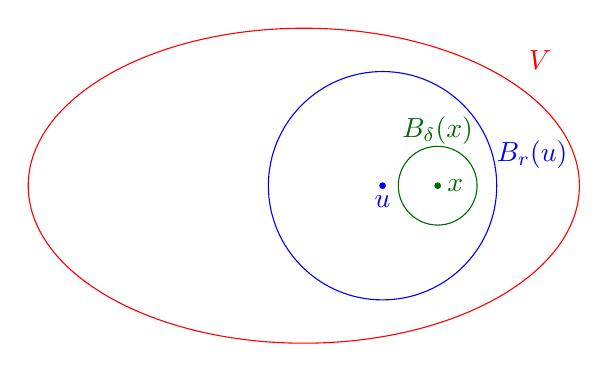
\begin{tikzpicture}
			\draw[red] (0,0) circle [x radius=3.5cm, y radius=2cm] ;
			\draw (3,1.6) node[red]{$V$};
			\draw [blue] (1,0) circle (1.45cm) ;
			\filldraw[blue] (1,0) circle (1pt) node[anchor=north]{$u$};
			\draw (2.9,0.4) node[blue]{$B_r(u)$};
			\draw [green!40!black] (1.7,0) circle (0.5cm) node [yshift=0.7cm]{$B_{\delta}(x)$} ;
			\filldraw[green!40!black] (1.7,0) circle (1pt) node[anchor=west]{$x$};
		\end{tikzpicture}
	\end{center}
\end{myproof}

\cor{}{By the result of the proof, we can then show...}

\mprop{}{$1 + 1 = 2$.}

\section{Random}
\dfn{Normed Linear Space and Norm $\boldsymbol{\|\cdot\|}$}{Let $V$ be a vector space over $\bbR$ (or $\bbC$). A norm on $V$ is function $\|\cdot\|\ V\to \bbR_{\geq 0}$ satisfying \begin{enumerate}[label=\bfseries\tiny\protect\circled{\small\arabic*}]
		\item \label{n:1}$\|x\|=0 \iff x=0$ $\forall$ $x\in V$
		\item \label{n:2}	$\|\lambda x\|=|\lambda|\|x\|$ $\forall$ $\lambda\in\bbR$(or $\bbC$), $x\in V$
		\item \label{n:3} $\|x+y\| \leq \|x\|+\|y\|$ $\forall$ $x,y\in V$ (Triangle Inequality/Subadditivity)
	\end{enumerate}And $V$ is called a normed linear space.

	$\bullet $ Same definition works with $V$ a vector space over $\bbC$ (again $\|\cdot\|\to\bbR_{\geq 0}$) where \ref{n:2} becomes $\|\lambda x\|=|\lambda|\|x\|$ $\forall$ $\lambda\in\bbC$, $x\in V$, where for $\lambda=a+ib$, $|\lambda|=\sqrt{a^2+b^2}$ }




\section{Algorithms}
\begin{algorithm}[H]
\KwIn{This is some input}
\KwOut{This is some output}
\SetAlgoLined
\SetNoFillComment
\tcc{This is a comment}
\vspace{3mm}
some code here\;
$x \leftarrow 0$\;
$y \leftarrow 0$\;
\uIf{$ x > 5$} {
    x is greater than 5 \tcp*{This is also a comment}
}
\Else {
    x is less than or equal to 5\;
}
\ForEach{y in 0..5} {
    $y \leftarrow y + 1$\;
}
\For{$y$ in $0..5$} {
    $y \leftarrow y - 1$\;
}
\While{$x > 5$} {
    $x \leftarrow x - 1$\;
}
\Return Return something here\;
\caption{what}
\end{algorithm}

\end{document}